\documentclass{standalone}
\usepackage{tikz}
\usetikzlibrary{patterns, positioning}

\begin{document}
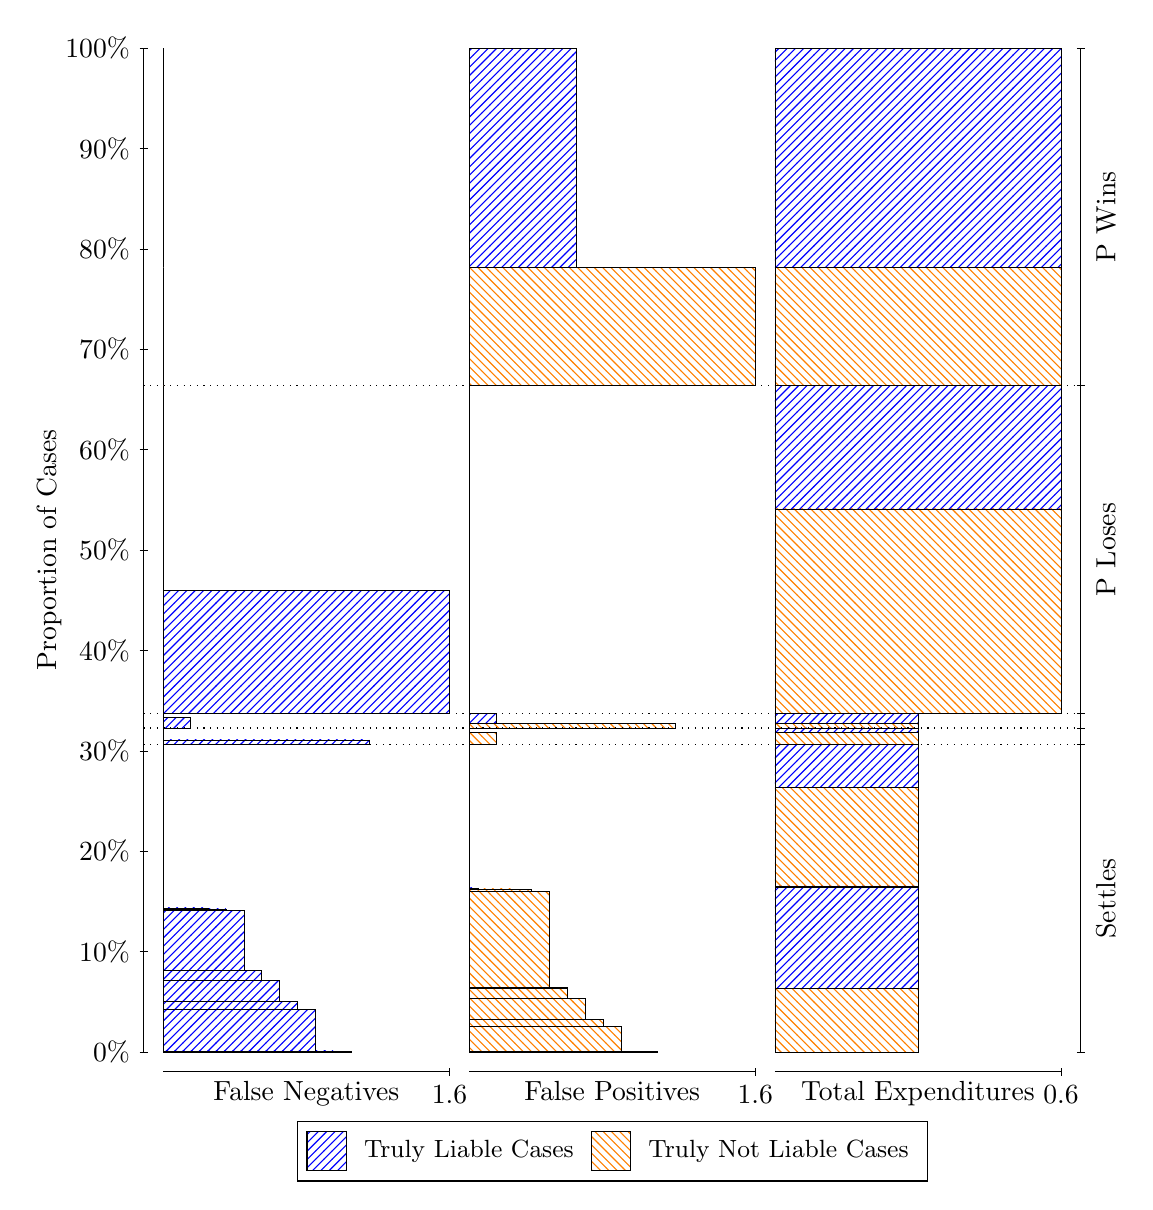
\begin{tikzpicture}
\draw[black, very thin] (1.5,1.75) -- (1.5,14.5);
\node[rotate=90, anchor=center] at (0.3, 8.125) {Proportion of Cases};
\draw[black, very thin] (1.45,1.75) -- (1.55,1.75);
\node[anchor=east] at (1.45, 1.75) {0\%};
\draw[black, very thin] (1.45,3.025) -- (1.55,3.025);
\node[anchor=east] at (1.45, 3.025) {10\%};
\draw[black, very thin] (1.45,4.3) -- (1.55,4.3);
\node[anchor=east] at (1.45, 4.3) {20\%};
\draw[black, very thin] (1.45,5.575) -- (1.55,5.575);
\node[anchor=east] at (1.45, 5.575) {30\%};
\draw[black, very thin] (1.45,6.85) -- (1.55,6.85);
\node[anchor=east] at (1.45, 6.85) {40\%};
\draw[black, very thin] (1.45,8.125) -- (1.55,8.125);
\node[anchor=east] at (1.45, 8.125) {50\%};
\draw[black, very thin] (1.45,9.4) -- (1.55,9.4);
\node[anchor=east] at (1.45, 9.4) {60\%};
\draw[black, very thin] (1.45,10.675) -- (1.55,10.675);
\node[anchor=east] at (1.45, 10.675) {70\%};
\draw[black, very thin] (1.45,11.95) -- (1.55,11.95);
\node[anchor=east] at (1.45, 11.95) {80\%};
\draw[black, very thin] (1.45,13.225) -- (1.55,13.225);
\node[anchor=east] at (1.45, 13.225) {90\%};
\draw[black, very thin] (1.45,14.5) -- (1.55,14.5);
\node[anchor=east] at (1.45, 14.5) {100\%};

\draw[black, very thin] (13.4,1.75) -- (13.4,14.5);
\draw[black, very thin] (13.35,1.75) -- (13.45,1.75);
\node[anchor=west] at (13.35, 1.75) {};
\draw[black, very thin] (13.35,5.6527) -- (13.45,5.6527);
\node[anchor=west] at (13.35, 5.6527) {};
\draw[black, very thin] (13.35,5.8646) -- (13.45,5.8646);
\node[anchor=west] at (13.35, 5.8646) {};
\draw[black, very thin] (13.35,6.0528) -- (13.45,6.0528);
\node[anchor=west] at (13.35, 6.0528) {};
\draw[black, very thin] (13.35,10.212) -- (13.45,10.212);
\node[anchor=west] at (13.35, 10.212) {};
\draw[black, very thin] (13.35,14.5) -- (13.45,14.5);
\node[anchor=west] at (13.35, 14.5) {};

\draw[black, very thin, pattern color=blue, pattern=north east lines] (1.75,1.75) rectangle (4.1344,1.7533);
\draw[black, very thin, pattern color=blue, pattern=north east lines] (1.75,1.7533) rectangle (3.9073,1.7642);
\draw[black, very thin, pattern color=blue, pattern=north east lines] (1.75,1.7642) rectangle (3.6802,2.2917);
\draw[black, very thin, pattern color=blue, pattern=north east lines] (1.75,2.2917) rectangle (3.4531,2.3896);
\draw[black, very thin, pattern color=blue, pattern=north east lines] (1.75,2.3896) rectangle (3.226,2.6618);
\draw[black, very thin, pattern color=blue, pattern=north east lines] (1.75,2.6618) rectangle (2.999,2.7852);
\draw[black, very thin, pattern color=blue, pattern=north east lines] (1.75,2.7852) rectangle (2.7719,3.5481);
\draw[black, very thin, pattern color=blue, pattern=north east lines] (1.75,3.5481) rectangle (2.5448,3.5677);
\draw[black, very thin, pattern color=blue, pattern=north east lines] (1.75,3.5677) rectangle (2.3177,3.5804);
\draw[black, very thin, pattern color=orange, pattern=north west lines] (1.75,3.5804) rectangle (1.75,5.6527);
\draw[black, very thin, pattern color=blue, pattern=north east lines] (1.75,5.6527) rectangle (4.3615,5.7131);
\draw[black, very thin, pattern color=orange, pattern=north west lines] (1.75,5.7131) rectangle (1.75,5.8646);
\draw[black, very thin, pattern color=blue, pattern=north east lines] (1.75,5.8646) rectangle (2.0906,5.9987);
\draw[black, very thin, pattern color=orange, pattern=north west lines] (1.75,5.9987) rectangle (1.75,6.0528);
\draw[black, very thin, pattern color=blue, pattern=north east lines] (1.75,6.0528) rectangle (5.3833,7.617);
\draw[black, very thin, pattern color=orange, pattern=north west lines] (1.75,7.617) rectangle (1.75,10.212);
\draw[black, very thin, pattern color=orange, pattern=north west lines] (1.75,10.212) rectangle (1.75,11.714);
\draw[black, very thin, pattern color=blue, pattern=north east lines] (1.75,11.714) rectangle (1.75,14.5);
\draw[black, very thin, pattern color=orange, pattern=north west lines] (5.6333,1.75) rectangle (8.0177,1.7543);
\draw[black, very thin, pattern color=orange, pattern=north west lines] (5.6333,1.7543) rectangle (7.7906,1.7622);
\draw[black, very thin, pattern color=orange, pattern=north west lines] (5.6333,1.7622) rectangle (7.5635,2.0757);
\draw[black, very thin, pattern color=orange, pattern=north west lines] (5.6333,2.0757) rectangle (7.3365,2.1627);
\draw[black, very thin, pattern color=orange, pattern=north west lines] (5.6333,2.1627) rectangle (7.1094,2.4327);
\draw[black, very thin, pattern color=orange, pattern=north west lines] (5.6333,2.4327) rectangle (6.8823,2.5623);
\draw[black, very thin, pattern color=orange, pattern=north west lines] (5.6333,2.5623) rectangle (6.8823,2.5672);
\draw[black, very thin, pattern color=orange, pattern=north west lines] (5.6333,2.5672) rectangle (6.6552,3.7854);
\draw[black, very thin, pattern color=orange, pattern=north west lines] (5.6333,3.7854) rectangle (6.4281,3.8123);
\draw[black, very thin, pattern color=orange, pattern=north west lines] (5.6333,3.8123) rectangle (6.201,3.8222);
\draw[black, very thin, pattern color=blue, pattern=north east lines] (5.6333,3.8222) rectangle (5.7469,3.8349);
\draw[black, very thin, pattern color=blue, pattern=north east lines] (5.6333,3.8349) rectangle (5.6333,5.6527);
\draw[black, very thin, pattern color=orange, pattern=north west lines] (5.6333,5.6527) rectangle (5.974,5.8042);
\draw[black, very thin, pattern color=blue, pattern=north east lines] (5.6333,5.8042) rectangle (5.6333,5.8646);
\draw[black, very thin, pattern color=orange, pattern=north west lines] (5.6333,5.8646) rectangle (8.2448,5.9186);
\draw[black, very thin, pattern color=blue, pattern=north east lines] (5.6333,5.9186) rectangle (5.974,6.0528);
\draw[black, very thin, pattern color=orange, pattern=north west lines] (5.6333,6.0528) rectangle (5.6333,8.6477);
\draw[black, very thin, pattern color=blue, pattern=north east lines] (5.6333,8.6477) rectangle (5.6333,10.212);
\draw[black, very thin, pattern color=orange, pattern=north west lines] (5.6333,10.212) rectangle (9.2667,11.714);
\draw[black, very thin, pattern color=blue, pattern=north east lines] (5.6333,11.714) rectangle (6.9958,14.5);
\draw[black, very thin, pattern color=orange, pattern=north west lines] (9.5167,1.75) rectangle (11.333,2.5623);
\draw[black, very thin, pattern color=blue, pattern=north east lines] (9.5167,2.5623) rectangle (11.333,3.8464);
\draw[black, very thin, pattern color=orange, pattern=north west lines] (9.5167,3.8464) rectangle (11.333,3.8564);
\draw[black, very thin, pattern color=blue, pattern=north east lines] (9.5167,3.8564) rectangle (11.333,3.8597);
\draw[black, very thin, pattern color=orange, pattern=north west lines] (9.5167,3.8597) rectangle (11.333,5.1097);
\draw[black, very thin, pattern color=blue, pattern=north east lines] (9.5167,5.1097) rectangle (11.333,5.6527);
\draw[black, very thin, pattern color=orange, pattern=north west lines] (9.5167,5.6527) rectangle (11.333,5.8042);
\draw[black, very thin, pattern color=blue, pattern=north east lines] (9.5167,5.8042) rectangle (11.333,5.8646);
\draw[black, very thin, pattern color=orange, pattern=north west lines] (9.5167,5.8646) rectangle (11.333,5.9186);
\draw[black, very thin, pattern color=blue, pattern=north east lines] (9.5167,5.9186) rectangle (11.333,6.0528);
\draw[black, very thin, pattern color=orange, pattern=north west lines] (9.5167,6.0528) rectangle (13.15,8.6477);
\draw[black, very thin, pattern color=blue, pattern=north east lines] (9.5167,8.6477) rectangle (13.15,10.212);
\draw[black, very thin, pattern color=orange, pattern=north west lines] (9.5167,10.212) rectangle (13.15,11.714);
\draw[black, very thin, pattern color=blue, pattern=north east lines] (9.5167,11.714) rectangle (13.15,14.5);
\draw[black, dotted] (1.5,5.6527) -- (13.4,5.6527);
\draw[black, dotted] (1.5,5.8646) -- (13.4,5.8646);
\draw[black, dotted] (1.5,6.0528) -- (13.4,6.0528);
\draw[black, dotted] (1.5,10.212) -- (13.4,10.212);
\draw[black, very thin] (1.75,1.5) -- (5.3833,1.5);
\node[anchor=north] at (3.5667, 1.5) {False Negatives};
\draw[black, very thin] (5.3833,1.45) -- (5.3833,1.55);
\node[anchor=north] at (5.3833, 1.45) {1.6};

\draw[black, very thin] (5.6333,1.5) -- (9.2667,1.5);
\node[anchor=north] at (7.45, 1.5) {False Positives};
\draw[black, very thin] (9.2667,1.45) -- (9.2667,1.55);
\node[anchor=north] at (9.2667, 1.45) {1.6};

\draw[black, very thin] (9.5167,1.5) -- (13.15,1.5);
\node[anchor=north] at (11.333, 1.5) {Total Expenditures};
\draw[black, very thin] (13.15,1.45) -- (13.15,1.55);
\node[anchor=north] at (13.15, 1.45) {0.6};

\node[black, centered, rotate=90] at (13.72, 3.7013) {Settles};


\node[black, centered, rotate=90] at (13.72, 8.1323) {P Loses};
\node[black, centered, rotate=90] at (13.72, 12.356) {P Wins};

\draw (7.449999999999999,1.5) node[draw=none] (baseCoordinate) {};
\begin{scope}[align=center]
        \matrix[scale=0.5, draw=black, below=0.5cm of baseCoordinate, nodes={draw}, column sep=0.1cm]{
            \node[rectangle, draw, minimum width=0.5cm, minimum height=0.5cm, pattern=north east lines, pattern color=blue] {}; &
            \node[draw=none, font=\small] (B) {Truly Liable Cases}; &
            \node[rectangle, draw, minimum width=0.5cm, minimum height=0.5cm, pattern=north west lines, pattern color=orange] {}; &
            \node[draw=none, font=\small] (B) {Truly Not Liable Cases}; \\
            };
\end{scope}

\end{tikzpicture}
\end{document}